\documentclass{article}

\usepackage{multirow}
\usepackage[utf8]{inputenc}
\usepackage{graphicx} % Required for the inclusion of images
\usepackage{natbib} % Required to change bibliography style to APA
\usepackage{mathtools}
\usepackage{listings}
\usepackage{color}
\usepackage[margin=1in]{geometry}
\usepackage[table,xcdraw]{xcolor}
\usepackage{multicol}
\usepackage{hyperref}
\usepackage{wrapfig}
\usepackage{capt-of}
\usepackage{caption}
\usepackage{subcaption}
\usepackage{wrapfig}
\usepackage{float}

\setlength\parindent{0pt} % Removes all indentation from paragraphs

\definecolor{dkgreen}{rgb}{0,0.6,0}
\definecolor{gray}{rgb}{0.5,0.5,0.5}
\definecolor{mauve}{rgb}{0.58,0,0.82}

\graphicspath{ {images/} }

\lstset{frame=tb,
  aboveskip=3mm,
  belowskip=3mm,
  showstringspaces=false,
  columns=flexible,
  basicstyle={\small\ttfamily},
  numbers=none,
  numberstyle=\tiny\color{gray},
  keywordstyle=\color{blue},
  commentstyle=\color{dkgreen},
  stringstyle=\color{mauve},
  breaklines=true,
  breakatwhitespace=true,
  tabsize=3
}

\title{Tutorial - GIT}

\author{Grupo de Linux da Universidade de Aveiro\\Eduardo Sousa - eduardosousa@ua.pt}

\date{2016}

\begin{document}

\maketitle

\section{Introduction}

Welcome to this tutorial. This is a brief introduction to version control software and GIT. This tutorial is separated in three parts:

\begin{itemize}
\item{Introduction}
\item{First steps}
\item{Advanced commands}
\end{itemize}

\textbf{Introduction} - we will talk about Version Control Systems and GIT.\\
\textbf{First steps} - we will talk about GIT's basic commands.\\
\textbf{Advanced commands} - we will talk about GIT's advanced commands.\\

\subsection{What is a version control system?}

A version control system (\textbf{VCS}) is a software that allows you to manage the changes in files, while retaining previous changes. It will also allow you to work with others more effectively, since it will track the changes for you.

\subsection{Why use version control system?}

Instead of using other kinds of systems, you can use \textbf{VCS} to track the changes in code and in file structure of your project. Just this aspect will allow you to focus in code production instead of always worrying if you have the right files or what others have changed in the files.

\subsection{What is GIT?}

\textbf{GIT} is one of the main \textbf{VCS} used for software development. \textbf{GIT} main goals are:

\begin{itemize}
\item{Speed}
\item{Data integrity}
\item{Distributed}
\item{Non-linear workflow}
\end{itemize}

GIT allows you to track your files and the changes made to them. GIT structures the tracking of files in a tree way, where each node of the tree will represent a different state of the repository. Each node of the GIT tree is called a commit and it is a snapshot of the files that where being tracked at the time of that commit. This tree structure allows you and your colleagues to see the different stages of the tree, in other words it represents the history of the project and the code.\\
The tree structure also allows for concurrent development, because each branch of the tree is independent and later the branches can be merged.

\begin{figure}[H]
\centerline{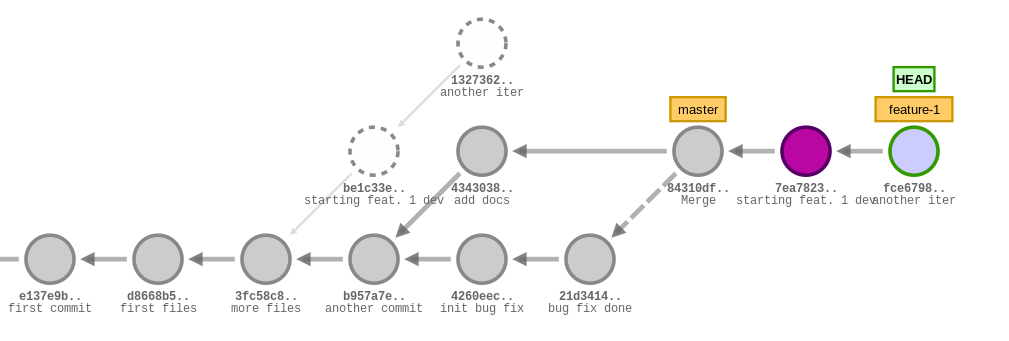
\includegraphics[scale=0.5]{repository_after_rebase.png}}
\caption{GIT tree structure}
\label{fig1}
\end{figure}

\section{First steps}

This is the beginning of a great journey for you. You will learn the basics of GIT, which will help until the end of your days as developer.

\subsection{Create a local repository}

First of all, lets create a new repository so you that you can start tracking all the changes in your project.

\begin{lstlisting}
	git init
	touch README.md
	git add README.md
	git commit -m "Initial commit"
\end{lstlisting}

Lets dissect each command:\\

\begin{itemize}
\item{\textbf{git init} - this command will initialize a local git repository in the folder you're in.}
\item{\textbf{touch README.md} - will create an empty file called README.md.}
\item{\textbf{git add README.md} - will make your local GIT repository start tracking your file.}
\item{\textbf{git commit -m "Initial commit"} - will set the actual state of the repository as the first snapshot taken.}
\end{itemize}

\begin{figure}[H]
\centerline{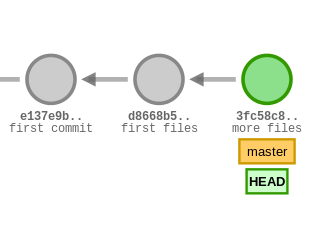
\includegraphics[scale=0.5]{initial_repository.png}}
\caption{Initial repository state}
\label{fig1}
\end{figure}

\subsection{Adding files}

Lets create a few other files so we can start tracking them with GIT.

\begin{lstlisting}
	touch file_1
	touch file_2
	mkdir folder_1
	touch folder_1/file_1
	touch folder_1/file_2
\end{lstlisting}

Lets check what is the state of the local GIT repository with \textbf{git status}.

\begin{lstlisting}
	On branch master
	Untracked files:
		(use "git add <file>..." to include in what will be committed)

	file_1
	file_2
	folder_1/

	nothing added to commit but untracked files present (use "git add" to track)
\end{lstlisting}

There are two ways of start tracking these files. You can add all files with one command or you can add them one by one. If you know that you want to add them all, you can use this command:

\begin{lstlisting}
	git add .
\end{lstlisting}

If you don't want to track all files, you can add them individually like this:

\begin{lstlisting}
	git add <file>
\end{lstlisting}

In this case, we want to add all files, so we will use \textbf{git add .} and know lets check the state of the local repository with \textbf{git status}.

\begin{lstlisting}
	On branch master
	Changes to be committed:
  		(use "git reset HEAD <file>..." to unstage)

	new file:   file_1
	new file:   file_2
	new file:   folder_1/file_1
	new file:   folder_1/file_2
\end{lstlisting}

\subsection{Making commits}

Now that we have added some new files and started tracking them in our repository, lets save this state. To save this changes in the repository, we need to make a commit of the changes. To commit the changes, we will use the following command:

\begin{lstlisting}
	git commit -m "A message relevant to the changes made in this commit"
\end{lstlisting}

Know that we know which command to use, lets use it but don't forget to add a meaningful message, so that when others check the commits to the repository can understand what or why you did those changes.\\

\subsection{Checking the log}

Lets check the log to see the changes we have made to our local repository. To check these changes, we will check the local repository log and to do that we must run the following command:

\begin{lstlisting}
	git log
\end{lstlisting}

After running this command, we will get an output similar to this:

\begin{lstlisting}
	commit 3070d3621b60b5ebe46b2d58ad6be2537069d79d
	Author: John Doe <john.doe@example.com>
	Date:   Tue Nov 15 15:44:20 2016 +0000

    	Added initial files

	commit 5814279838033e7b0f14a620c73202f52f11cf99
	Author: John Doe <john.doe@example.com>
	Date:   Tue Nov 15 15:26:39 2016 +0000

    	Initial commit
\end{lstlisting}

What can we check in the log? Well, we can see the commits that were made to the repository, when were they made and the message that the author of the commit wrote for that change.\\

Now lets say you want to check what a specific commit made. You can verify this with this command:

\begin{lstlisting}
	git show <commit hash>
\end{lstlisting}

Where the \textbf{\textless commit hash\textgreater} is the number that appears after the commit word when using the \textbf{git log}.\\

\subsection{Updating the remote server}

% TODO: Updating the remote server
% Code.UA vs GitHub

\subsection{Creating a branch}

GIT supports branches. What are branches? Branches are places where code diverges, meaning that the code will have the same base, but it will differ from branch to branch. Every GIT repository has main branch, that is called master and if you don't branch all your commits will go there.\\

Now lets say you need to add a new feature. You don't want to break the master branch while you develop your new feature, so you will create a new branch so that you can work on code. To create the new branch, you will use the following command:

\begin{lstlisting}
	git branch <branch name>
\end{lstlisting}

Lets create a new branch for our new feature called \textbf{feature-1}. After creating your new branch to work on you should check in which branch are you in, by running the following command \textbf{git branch}. And you will get the following result:

\begin{lstlisting}
	  feature-1
	* master
\end{lstlisting}

\begin{figure}[H]
\centerline{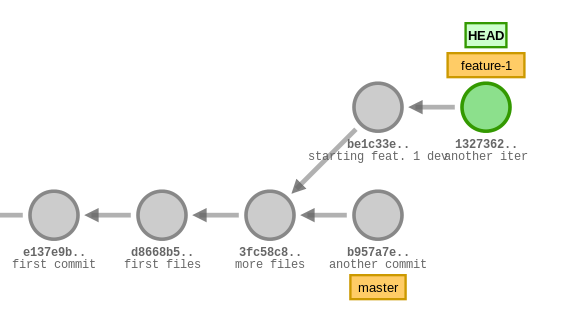
\includegraphics[scale=0.5]{repository_after_branch.png}}
\caption{Repository after creating branch feature-1}
\label{fig1}
\end{figure}

The star (*) before the name of the branch will tell you which in which branch you are and right now you should be in the master branch. But we want to develop our new feature, so we will need to change to the feature-1 branch. To do that we need to run the following command:

\begin{lstlisting}
	git checkout <branch name>
\end{lstlisting}

After we run this command you should check in which branch are you now and the result should be feature-1 as demonstrated in the following:

\begin{lstlisting}
	* feature-1
	  master
\end{lstlisting}

Now we can develop our feature in this branch, without changing the master branch.\\
Lets add a new file called feat\_1 and lets add and commit our new feature to the repository. Lets do this by running the following commands:

\begin{lstlisting}
	echo "feature 1 developed" >> file_1
	git add file_1
	git commit -m "Feature 1 complete"
	git log
\end{lstlisting}

And the output should be similar to this:

\begin{lstlisting}
	commit 43756632d9dedf6b8756e1dd393d877ee7c81a4d
	Author: John Doe <john.doe@example.com>
	Date:   Tue Nov 15 16:55:18 2016 +0000

    	Feature 1 complete

	commit 3070d3621b60b5ebe46b2d58ad6be2537069d79d
	Author: John Doe <john.doe@example.com>
	Date:   Tue Nov 15 15:44:20 2016 +0000

    	Added initial files

	commit 5814279838033e7b0f14a620c73202f52f11cf99
	Author: John Doe <john.doe@example.com>
	Date:   Tue Nov 15 15:26:39 2016 +0000

    	Initial commit
\end{lstlisting}

So now our code in feature-1 branch as a new feature that the master branch doesn't have. Lets just check our master branch to check that the change that we made didn't made it to the master branch, by running the following commands:

\begin{lstlisting}
	git checkout master
	git log
\end{lstlisting}

The result should be similar to this:

\begin{lstlisting}
	commit 3070d3621b60b5ebe46b2d58ad6be2537069d79d
	Author: John Doe <john.doe@example.com>
	Date:   Tue Nov 15 15:44:20 2016 +0000

    	Added initial files

	commit 5814279838033e7b0f14a620c73202f52f11cf99
	Author: John Doe <john.doe@example.com>
	Date:   Tue Nov 15 15:26:39 2016 +0000

    	Initial commit
\end{lstlisting}

As we can see in the last output, the master branch didn't get changed, while the changes we did are saved in the feature-1 branch.\\

\subsection{Merge vs Rebase}

Run this code in your terminal so that the repository matches the next exercise:

\begin{lstlisting}
	git checkout master
	git branch bug_fix_1
	git checkout bug_fix_1
	echo "this is a bug fix" >> file_1
	git commit -a -m "Bug Fix 1 solved"
	git checkout master
\end{lstlisting}

Now we want to do a lot of things with our repository. We have two things happening, we developed our feature 1 and one of our colleagues developed a bug fix for a bug found in the master branch. Our colleague did his bug fix on the branch bug\_fix\_1.\\

\begin{figure}[H]
\centerline{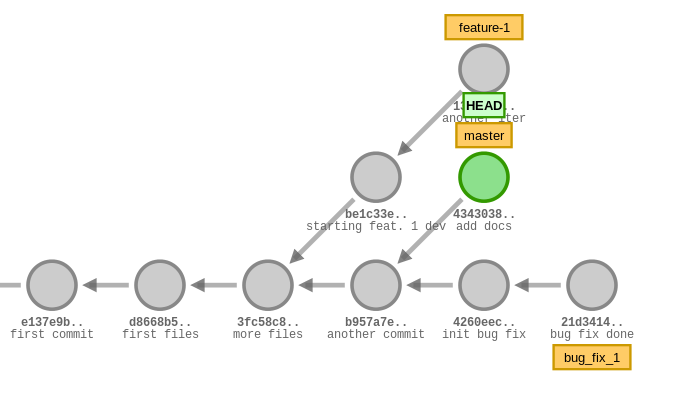
\includegraphics[scale=0.5]{repository_with_3_branches.png}}
\caption{State of the repository after another branch has been created}
\label{fig1}
\end{figure}

There are two kinds of operations: 

\begin{itemize}
	\item{\textbf{Merge} - this operation will join two commits from different branches in a new commit in the branch you are}
	\item{\textbf{Rebase} - this operation will take the commits in one branch and apply them before the commits of the branch you are in}
\end{itemize}

\subsubsection{Merge}

So now we want to merge the bug fix into the master branch because we want our master branch to have the less amount of bugs possible. To do this, first we must check if we are in the master branch and then merge the bug\_fix\_1 branch into the master branch. To check if we are in the correct branch we need to run \textbf{git branch} and the output is:

\begin{lstlisting}
	  bug_fix_1
	  feature-1
	* master
\end{lstlisting}

If this isn't your case you need to run \textbf{git checkout master}.\\

After doing all this, the last thing that we need to do to merge both branches is:

\begin{lstlisting}
	git merge bug_fix_1
\end{lstlisting}

Since we merged the two branches, both of them should be equal. To check that all the commits have made into master branch lets check the log, by running \textbf{git log}:

\begin{lstlisting}
	commit 3b820eeb454915a81373a569a8a4baf32a6725b1
	Author: John Doe <john.doe@example.com>
	Date:   Tue Nov 15 21:31:43 2016 +0000

    	Bug fix 1 solved

	commit 3070d3621b60b5ebe46b2d58ad6be2537069d79d
	Author: John Doe <john.doe@example.com>
	Date:   Tue Nov 15 15:44:20 2016 +0000

    	Added initial files

	commit 5814279838033e7b0f14a620c73202f52f11cf99
	Author: John Doe <john.doe@example.com>
	Date:   Tue Nov 15 15:26:39 2016 +0000

    	Initial commit
\end{lstlisting}

\begin{figure}[H]
\centerline{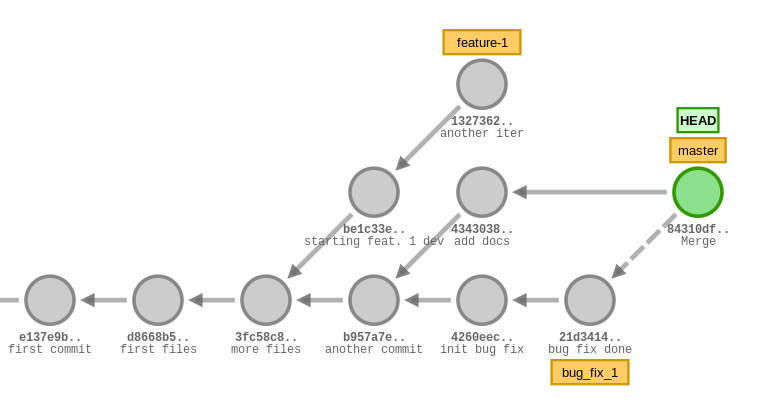
\includegraphics[scale=0.5]{repository_after_merge.png}}
\caption{Repository state after the merge}
\label{fig1}
\end{figure}

And lets check if the last commit is the same in both branches, by running \textbf{git branch -v}:

\begin{lstlisting}
	  bug_fix_1 3b820ee Bug fix 1 solved
	  feature-1 4375663 Feature 1 complete
	* master    3b820ee Bug fix 1 solved
\end{lstlisting}

Now that the bug\_fix\_1 branch has been merged into the master branch, we don't need that branch anymore, so lets delete it. To do this run:

\begin{lstlisting}
	git branch -d bug_fix_1
\end{lstlisting}

And now lets check that we did in fact deleted the bug\_fix\_1 branch and that we didn't lose any information by running again \textbf{git branch -v}:

\begin{lstlisting}
	  feature-1 4375663 Feature 1 complete
	* master    3b820ee Bug fix 1 solved
\end{lstlisting}

\begin{figure}[H]
\centerline{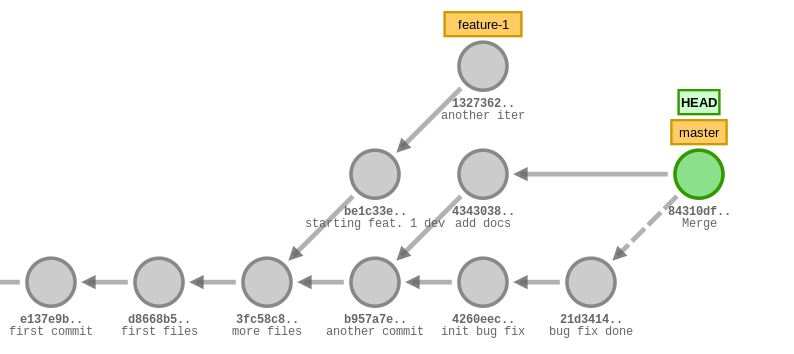
\includegraphics[scale=0.5]{repository_after_deleting_branch.png}}
\caption{Repository state after deleting branch}
\label{fig1}
\end{figure}

\subsubsection{Rebase}

Now we want to update our feature-1 branch with the latest code from the master branch, to check if the bug fix that we merged into the master branch won't insert any bugs when merged with our new feature. To do this we must change to our feature-1 branch and then rebase it with the commits from the master branch.

\begin{lstlisting}
	git checkout feature-1
	git rebase master
\end{lstlisting}

And the output should be something like this:

\begin{lstlisting}
	Auto-merging file_1
	CONFLICT (content): Merge conflict in file_1
	Recorded preimage for 'file_1'
	Automatic merge failed; fix conflicts and then commit the result.
\end{lstlisting}

Since we changed the same file in both branches, we need to fix this. Open the file with vim, using the following command \textbf{vim file\_1}. The file should be similar to this:

\begin{lstlisting}
	<<<<<<< HEAD
	feature 1 developed
	=======
	this is a bug fix
	>>>>>>> master
\end{lstlisting}

Now we must decide what to keep, so lets fix the file, by keeping what we want to keep and removing what is not needed, including \textbf{\textless\textless\textless\textless\textless\textless\textless\textless HEAD} and \textbf{\textgreater\textgreater\textgreater\textgreater\textgreater\textgreater\textgreater\textgreater master}. By the end of this conflict resolution, we should have a file equal to this:

\begin{lstlisting}
	this is a bug fix
	feature 1 developed
\end{lstlisting}

Now lets add the file and commit the rebase fix:

\begin{lstlisting}
	git add file_1
	git commit -m "Fixing rebase errors"
\end{lstlisting}

Now lets check the history of this branch by running \textbf{git log}.

\begin{lstlisting}
	commit c7cbf0e80fb8564f5cfa5a9f7d20f2002fb7847b
	Merge: 76a5e9e 3b820ee
	Author: John Doe <john.doe@example.com>
	Date:   Tue Nov 15 23:59:40 2016 +0000

    	Fixing rebase errors

	commit 76a5e9efc2c59ff487fae6636c9eeb80720ab541
	Author: John Doe <john.doe@example.com>
	Date:   Tue Nov 15 23:49:28 2016 +0000

    	Feature 1 complete

	commit 3b820eeb454915a81373a569a8a4baf32a6725b1
	Author: John Doe <john.doe@example.com>
	Date:   Tue Nov 15 21:31:43 2016 +0000

    	Bug fix 1 solved

	commit 3070d3621b60b5ebe46b2d58ad6be2537069d79d
	Author: John Doe <john.doe@example.com>
	Date:   Tue Nov 15 15:44:20 2016 +0000

    	Added initial files

	commit 5814279838033e7b0f14a620c73202f52f11cf99
	Author: John Doe <john.doe@example.com>
	Date:   Tue Nov 15 15:26:39 2016 +0000

    	Initial commit
\end{lstlisting}

\begin{figure}[H]
\centerline{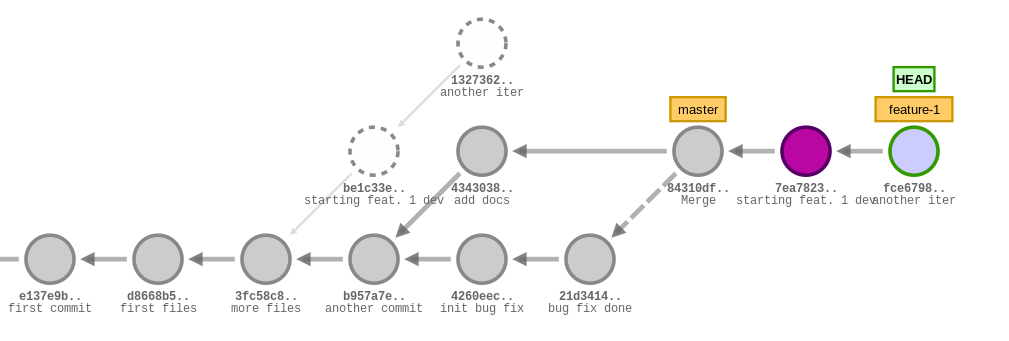
\includegraphics[scale=0.5]{repository_after_rebase.png}}
\caption{Repository state after rebase}
\label{fig1}
\end{figure}

\subsection{Reset}

Lets say that we did an error when we fixed the rebase error, how can we undo it? Simple we can use \textbf{git reset HEAD~N}, where \textbf{N} represents the number of commits that we want to reset to. Since we only want to undo the last commit we will use N = 1.

\begin{lstlisting}
	git reset HEAD~1
\end{lstlisting}

To check that the \textbf{git reset} was successful, lets run \textbf{git log}.

\begin{lstlisting}
	commit 76a5e9efc2c59ff487fae6636c9eeb80720ab541
	Author: John Doe <john.doe@example.com>
	Date:   Tue Nov 15 23:49:28 2016 +0000

    	Feature 1 complete

	commit 3070d3621b60b5ebe46b2d58ad6be2537069d79d
	Author: John Doe <john.doe@example.com>
	Date:   Tue Nov 15 15:44:20 2016 +0000

    	Added initial files

	commit 5814279838033e7b0f14a620c73202f52f11cf99
	Author: John Doe <john.doe@example.com>
	Date:   Tue Nov 15 15:26:39 2016 +0000

    	Initial commit
\end{lstlisting}

We can now check that the rebase never happened.

\section{Advanced tricks}

\subsection{Cherry-pick}

\subsection{RefLog}

\subsection{Bisect}

\subsection{}

\end{document}
